\documentclass[12pt]{article}
\usepackage[a4paper, left=1.9cm, right=1.9cm, top=2.5cm, bottom=2.5cm]{geometry}
\usepackage{hyperref}
\usepackage{colortbl}
\usepackage[export]{adjustbox}
\usepackage{graphicx}
\usepackage{listings}
\usepackage[T1]{fontenc}
\usepackage{lmodern}
\usepackage{microtype}
\DisableLigatures[-]{}
\usepackage{enumitem}
\graphicspath{ {./media/} }
%\def\darktheme{0}  % Comment this line to toggle dark theme
\usepackage[italian]{babel}
\usepackage{tocloft}
\usepackage[table]{xcolor}
\usepackage{pagecolor}
\usepackage{parskip}
\usepackage{environ}
\usepackage[most]{tcolorbox}
\usepackage{titlesec}
\usepackage[dotinlabels]{titletoc}

\titleformat{\section}[hang]{\bfseries\Large}{\thesection.}{0.5em}{}

\appto\appendix{%
  \setcounter{secnumdepth}{-2}
  \addtocontents{toc}{%
    \unexpanded{\unexpanded{%
        \cftpagenumbersoff{section}%
        \setlength\cftsecindent{\cftsecnumwidth}%
      }}%
  }%
}

\renewcommand{\cftsecleader}{\cftdotfill{\cftdotsep}}
\addto\captionsitalian{
  \renewcommand{\contentsname}%
  {Indice}%
}

\ifx\darktheme\undefined
  \definecolor{bcolor}{RGB}{255,255,255}
  \definecolor{textcolor}{RGB}{0,0,0}
  \definecolor{linkcolor}{RGB}{0, 0, 255}
  \definecolor{tblhdrcolor}{gray}{0.8}
  \definecolor{tmpltbcolot}{gray}{0.9}
\else
  \definecolor{bcolor}{RGB}{41,41,41}
  \definecolor{textcolor}{RGB}{255,255,255}
  \definecolor{linkcolor}{RGB}{0, 167, 255}
  \definecolor{tblhdrcolor}{RGB}{69, 69, 69}
  \definecolor{tmpltbcolot}{RGB}{69, 69, 69}
\fi

\pagecolor{bcolor}
\color{textcolor}

\newtcolorbox{templateblock}{
  colupper=textcolor,
  colback=tmpltbcolot,
  boxrule=0pt,
  boxsep=0pt,
  breakable}

\hypersetup{
  colorlinks=true,
  linkcolor=textcolor,
  urlcolor=linkcolor}

\urlstyle{same}

\lstdefinestyle{customc}{
  basicstyle=\footnotesize\ttfamily,
  belowcaptionskip=1\baselineskip,
  breaklines=true,
  language=C,
  commentstyle=\color{green!50!black},
  keywordstyle=\color{blue},
  stringstyle=\color{red!55!black!92!white},
  directivestyle=\bfseries\color{gray},
  numbers=left,
  numbersep=5pt,
  numberstyle=\tiny\color{black},
  showstringspaces=false,
  stepnumber=1,
  tabsize=2,
  title=\lstname,
}

\lstdefinestyle{customcxx}{
  basicstyle=\footnotesize\ttfamily,
  belowcaptionskip=1\baselineskip,
  breaklines=true,
  language=C++,
  commentstyle=\color{green!50!black},
  keywordstyle=\color{blue},
  stringstyle=\color{red!55!black!92!white},
  directivestyle=\bfseries\color{gray},
  numbers=left,
  numbersep=5pt,
  numberstyle=\tiny\color{black},
  showstringspaces=false,
  stepnumber=1,
  tabsize=2,
  title=\lstname,
}

\lstdefinestyle{customsql}{
  basicstyle=\footnotesize\ttfamily,
  belowcaptionskip=1\baselineskip,
  breaklines=true,
  language=SQL,
  commentstyle=\color{green!50!black},
  keywordstyle=\color{blue},
  stringstyle=\color{red!55!black!92!white},
  numbers=left,
  numbersep=5pt,
  numberstyle=\tiny\color{black},
  showstringspaces=false,
  stepnumber=1,
  tabsize=2,
  title=\lstname,
}
\newcommand{\inputcfile}[1]{{
      \lstset{mathescape=false, escapechar=, style=customc}
      \lstinputlisting[language=C]{#1}
      \pagebreak}}

\newcommand{\inputcxxfile}[1]{{
      \lstset{mathescape=false, escapechar=, style=customcxx}
      \lstinputlisting[language=C++]{#1}
      \pagebreak}}

\newcommand{\inputsqlfile}[1]{{
      \lstset{mathescape=false, escapechar=, style=customsql}
      \lstinputlisting[language=SQL]{#1}}}

\counterwithin*{figure}{subsection}
\counterwithin*{table}{subsection}
% * means don't change the representation, because we'll do it now
\renewcommand{\thefigure}{%
  \ifnum\value{subsubsection}>0
    \thesubsubsection.%
  \else
    \ifnum\value{subsection}>0
      \thesubsection.%
    \else
      \thesection.%
    \fi
  \fi
  \arabic{figure}%
}
\renewcommand{\thetable}{%
  \ifnum\value{subsubsection}>0
    \thesubsubsection.%
  \else
    \ifnum\value{subsection}>0
      \thesubsection.%
    \else
      \thesection.%
    \fi
  \fi
  \arabic{table}%
}
\usepackage{anyfontsize}

\makeatletter
\def\authorid#1{\gdef\@authorid{#1}}
\def\@authorid{\@latex@warning@no@line{No \noexpand\authorid given}}
\makeatother

\makeatletter
\def\authorname#1{\gdef\@authorname{#1}}
\def\@authorname{\@latex@warning@no@line{No \noexpand\authorname given}}
\makeatother

\makeatletter
\def\authorsurname#1{\gdef\@authorsurname{#1}}
\def\@authorsurname{\@latex@warning@no@line{No \noexpand\authorsurname given}}
\makeatother

\makeatletter
\def\@maketitle{%
    \null
    \begin{center}%
        \let \footnote \thanks
        {\fontsize{16}{18}\selectfont
            \vskip 1.5em%
            Ingegneria di Internet e del Web \\
            \vskip 1em%
            Progetto B1 A.A. 2019/2020 \\}
        \vskip 5em%
            {\fontsize{20}{22}\selectfont \@title \par}%
            {\vskip 5em%
                \lineskip .5em%
                \fontsize{20}{22}\selectfont
                \@authorid \\
                \vskip 1em%
                \@authorname \ \@authorsurname \par}%
        \vskip 1em%
    \end{center}%
    \par
    \vskip 3em}
\makeatother

\usepackage{fancyhdr}

\makeatletter
\fancypagestyle{plain}{%
    \renewcommand{\headrulewidth}{0pt}
    \fancyhf{}
    \fancyhead[L]{\textit{\@authorid}}
    \fancyhead[C]{\@authorsurname \ \@authorname}
    \fancyhead[R]{Ingegneria di Internet e del Web}
    \fancyfoot[C]{\thepage}
}
\makeatother
\pagestyle{plain}

\usepackage{tikz}
\usetikzlibrary{arrows.meta, positioning, automata}
\usepackage{algorithm}
\usepackage{algorithmicx}
\usepackage{algpseudocode}

% La relazione deve contenere:
% - la descrizione dettagliata dell'architettura del sistema e delle scelte
%   progettuali effettuate;
% - la descrizione dell'implementazione;
% - la descrizione delle eventuali limitazioni riscontrate;
% - l'indicazione della piattaforma software usata per lo sviluppo ed il
%   testing del sistema;
% - alcuni esempi di funzionamento;
% - valutazione delle prestazioni del protocollo al variare della dimensione
%   della finestra di spedizione N, della probabilità di perdita dei messaggi p,
%   e della durata del timeout T (incluso il caso di T adattativo)
% - un manuale per l'installazione, la configurazione e l'esecuzione del
%   sistema.
\title{\uppercase{Trasferimento file su UDP}}
\authorid{0253822}
\authorname{Fabio}
\authorsurname{Buracchi}
\begin{document}

\includegraphics[width=2.1cm, valign=t]{image1}
\hfill

\includegraphics[width=3.55cm, valign=t]{image2}
{\let\newpage\relax\maketitle}
\tableofcontents
\pagebreak
\section{Requisiti} {

Lo scopo del progetto è quello di progettare ed implementare in linguaggi C
usando l'API del socket di Berkeley un'applicazione client-server per il
trasferimento di file che impieghi il servizio di rete senza connessione
(socket tipo SOCK\_DGRAM, ovvero UDP come protocollo di strato di trasporto.)
Il software deve permettere:

\begin{itemize}
    \item Connessione client-server senza autenticazione;
    \item La visualizzazione sul client dei file disponibili sul server
          (comando list);
    \item Il download di un file dal server (comando get);
    \item L'upload di un file sul server (comando put);
    \item Il trasferimento file in modo affidabile.
\end{itemize}

La comunicazione tra client e server deve avvenire tramite un opportuno
protocollo. Il protocollo di comunicazione deve prevedere lo scambio di due
tipi di messaggi:

\begin{enumerate}
    \item messaggi di comando: vengono inviati dal client al server per
          richiedere l'esecuzione delle diverse operazioni
    \item messaggi di risposta: vengono inviati dal server al client in risposta
          ad un comando con l'esito dell'operazione.
\end{enumerate}

\subsection{Funzionalità del server}

Il server, di tipo concorrente, deve fornire le seguenti funzionalità:

\begin{itemize}
    \item L'invio del messaggio di risposta al comando list al client
          richiedente; il messaggio di risposta contiene la filelist, ovvero la
          lista dei nomi dei file disponibili per la condivisione;
    \item L'invio del messaggio di risposta al comando get contenente il file
          richiesto, se presente, o un opportuno messaggio di errore;
    \item La ricezione di un messaggio put contenente il file da caricare sul
          server e l'invio di un messaggio di risposta con l'esito
          dell'operazione.
\end{itemize}

\subsection{Funzionalità del client}

I client, di tipo concorrente, devono fornire le seguenti funzionalità:

\begin{itemize}
    \item L'invio del messaggio list per richiedere la lista dei nomi dei file
          disponibili;
    \item L'invio del messaggio get per ottenere un file
    \item La ricezione di un file richiesta tramite il messaggio di get o la
          gestione dell'eventuale errore
    \item L'invio del messaggio put per effettuare l'upload di un file sul
          server e la ricezione del messaggio di risposta con l'esito
          dell'operazione.
\end{itemize}

\pagebreak
\subsection{Trasmissione affidabile}

Lo scambio di messaggi avviene usando un servizio di comunicazione non
affidabile. Al fine di garantire la corretta spedizione/ricezione dei messaggi
e dei file sia i client che il server implementano a livello applicativo il
protocollo Go-Back N
(cfr. Kurose \& Ross “Reti di Calcolatori e Internet”, 7° Edizione).

Per simulare la perdita dei messaggi in rete (evento alquanto improbabile in
una rete locale per non parlare di quando client e server sono eseguiti sullo
stesso host), si assume che ogni messaggio sia scartato dal mittente con
probabilità $p$.

La dimensione della finestra di spedizione $N$, la probabilità di perdita dei
messaggi $p$, e la durata del timeout $T$, sono tre costanti configurabili
ed uguali per tutti i processi. Oltre all'uso di un timeout fisso, deve essere
possibile scegliere l'uso di un valore per il timeout adattivo calcolato
dinamicamente in base alla evoluzione dei ritardi di rete osservati.

I client ed il server devono essere eseguiti nello spazio utente senza
richiedere privilegi di root. Il server deve essere in ascolto su una porta
di default (configurabile).

}
\section{Architettura} {

% descrizione dettagliata dell'architettura del sistema e delle scelte
% progettuali effettuate

\subsection{Protocollo TFTP}

Il "Trivial File Transfer Protocol" (TFTP) è un protocollo semplice per il trasferimento di file, definito nell'RFC 1350, che consente ad un client di ottenere o inviare file verso un host remoto.
Tale protocollo è progettato per essere implementato su UDP ed è equivalente al protocollo Stop-and-wait ARQ in termini di modalità di trasferimento dei pacchetti.

TFTP non include alcun meccanismo di controllo per l'autenticazione, per l'accesso, la riservatezza o la verifica dell'integrità dei dati. È necessario prestare attenzione ai diritti concessi a un processo server TFTP in modo da non violare la sicurezza del file system dell'host su cui è eseguito il processo.
I server TFTP vengono generalmente configurati con privilegi tali da permettere il solo accesso in lettura dei file.
A causa di tali considerazioni sulla sicurezza, il protocollo TFTP non trova generalmente applicazione nelle reti internet, mentre è principalmente utilizzato nelle reti locali (LAN) per operazioni come il trasferimento di immagini di avvio per nodi senza disco.

Un aspetto rilevante riguardo alle estensioni del protocollo, descritto nell'RFC 7440, riguarda l'introduzione di un'opzione che permette a client e server di negoziare una finestra di blocchi consecutivi da inviare, anziché utilizzare il tradizionale schema lockstep, al fine di migliorare il throughput complessivo. Tale estensione rende l'operazione di trasferimento di pacchetti equivalente a quella descritta dal protocollo Go-Back-N ARQ.

La scelta di adottare TFTP in questo progetto si fonda quindi su due motivazioni principali:
\begin{itemize}
    \item \textbf{Semplicità:} TFTP garantisce una semplice implementazione rispettando i requisiti progettuali.
    \item \textbf{Utilità:} Rispetto allo sviluppo di un protocollo ex novo, utilizzare un protocollo standardizzato e popolare come TFTP massimizza la possibilità di riutilizzo del sistema sviluppato, oltre ad offrire una maggiore interoperabilità con sistemi e strumenti esistenti.
\end{itemize}

In sintesi, TFTP rappresenta una soluzione concreta e realizzabile per lo sviluppo di un'applicazione di trasferimento file utile, adatta a contesti reali e soddisfacente i requisiti progettuali.

\subsubsection{Estensioni al protocollo TFTP}

Il protocollo TFTP non prevede meccanismi di timeout adattivo o un comando per ottenere l'elenco dei file disponibili su cui eseguire operazioni di lettura.
È stata dunque implementata un'estensione del protocollo TFTP con le seguenti modifiche:

\begin{itemize}
    \item \textbf{Timeout adattivo:} È stata introdotta la possibilità di richiedere l'uso di un timeout adattivo per le richieste di lettura (RRQ). Ciò avviene specificando il valore \texttt{adaptive} per l'opzione \texttt{timeout} definita nell'RFC 2349. In questo modo, il server utilizzerà un algoritmo di timeout adattivo basato su stime dinamiche del Round-Trip Time (RTT).
    
    \item \textbf{Richiesta elenco file:} Per ottenere la lista dei file scaricabili, è possibile inviare una richiesta RRQ con l'opzione chiave-valore case insensitive \texttt{type:directory}.
    Il server, in risposta, restituirà l'elenco dei file disponibili nel percorso relativo specificato nel campo \texttt{filename}.
\end{itemize}

\subsection{Server}

Il server TFTP è un'applicazione single-process multi-threaded che gestisce in maniera isolata e concorrente le sessioni di comunicazione con i client.

Il server, al momento della sua inizializzazione, crea un numero configurabile di \emph{worker thread} gestiti in una \emph{worker pool}.
Ciascun worker thread gestisce simultaneamente un numero massimo configurabile di sessioni.
Le richieste dei client in ingresso vengono assegnate ad un worker utilizzando un algoritmo di bilanciamento del carico, in modo tale da ottimizzare l'utilizzo delle risorse.

Il thread principale si occupa di gestire le richieste in arrivo, creando una nuova sessione per ogni richiesta valida. La versione del protocollo Internet utilizzata dalla socket, impiegata dal thread principale per la ricezione dei pacchetti dai client, è configurabile. Assegnando alla socket un indirizzo IPv4, il server gestirà esclusivamente richieste IPv4. Al contrario, se viene assegnato un indirizzo IPv6, il server sarà in grado di gestire sia richieste IPv6 che IPv4, creando in quest'ultimo caso sessioni basate su connessioni IPv4 per supportare eventuali client che non supportano il protocollo IPv6.

Ciascun worker thread gestisce un ciclo di eventi basato sul multiplexing dell'I/O, che consente l'esecuzione di operazioni non bloccanti. In questo contesto, il ciclo non si limita a monitorare simultaneamente più canali di I/O, ma integra anche la gestione dei timeout.

È possibile abilitare il supporto, disabilitato per default per ragioni di sicurezza, alle:
\begin{itemize}
    \item richieste di scrittura
    \item richieste di lettura della lista dei file di una directory
    \item richieste di lettura utilizzando un timeout adattivo
\end{itemize}

Il server integra un sistema di monitoraggio in grado di raccogliere dati statistici sia a livello di processo che di singola sessione. Questa funzionalità permette di analizzare in dettaglio e registrare l'andamento delle comunicazioni, agevolando il controllo del corretto funzionamento e la diagnosi di eventuali anomalie e facilitando l'integrazione del prodotto con applicazioni di terze parti.

\subsection{Client}

Il client TFTP è un'applicazione single-process e single-threaded.
È supportata la configurazione della versione del protocollo Internet (IPv4 o IPv6) utilizzata per la comunicazione, garantendo così la compatibilità con diversi ambienti di rete.
Poiché il protocollo TFTP non consente di effettuare trasferimenti multipli in una singola sessione, il client è stato progettato per operare in modalità non interattiva. Questa scelta riduce il consumo delle risorse, ad esempio minimizzando il tempo di occupazione del canale di comunicazione del server.

\subsection{Timeout adattivo}

Il timeout adattivo del server è stato progettato ispirandosi all'RFC 6298, che definisce l'algoritmo standard per il calcolo del timer di ritrasmissione nel protocollo TCP. Tuttavia, considerando l'impiego in una rete locale e l'uso con applicazioni TFTP, dove la congestione non rappresenta un problema significativo, sono state adottate durate iniziali e massime inferiori per il timeout. Il sistema utilizza una media esponenziale per stimare il Round-Trip Time (RTT), come descritto da Van Jacobson nel suo lavoro sul controllo della congestione, e applica un backoff esponenziale in caso di ritrasmissioni successive. Inoltre, l'algoritmo di Karn viene implementato per evitare che le misurazioni del RTT siano influenzate da ritrasmissioni, garantendo così una stima più accurata dei tempi di risposta.

}
\section{Implementazione} {

% descrizione dell'implementazione

Il prodotto finale si articola nei seguenti componenti:
\begin{itemize}
    \item Un eseguibile, dotato di interfaccia a riga di comando, che implementa il server TFTP.
    \item Un eseguibile, anch'esso con interfaccia a riga di comando, destinato a svolgere il ruolo di client TFTP.
    \item Una libreria statica, denominata \texttt{tftp}, che raccoglie la logica del protocollo. Essa è distribuita insieme a file di intestazione in linguaggio C costituendo un'API completa per lo sviluppo di soluzioni basate sul protocollo TFTP.
    \item Una libreria statica, \texttt{logger} progettata per gestire il logging degli eventi.
\end{itemize}

Tutti i componenti sono stati sviluppati integralmente in linguaggio ISO C23 per piattaforme Linux, ad eccezione degli eseguibili, che includono anche sorgenti in linguaggio ISO C++23 costituenti un livello di compatibilità necessario a sfruttare la libreria \texttt{CLI11} per la realizzazione dell'interfaccia a riga di comando, in quanto le più popolari librerie C per il parsing degli argomenti si sono dimostrate inadeguate.

È notevole osservare che, oltre ad introdurre utili costrutti come l'inizializzatore vuoto (\texttt{=\{\}}), gli attributi, il supporto per etichette seguite da dichiarazioni e la nuova keyword \texttt{nullptr}, lo standard ISO/IEC 9899:2024 corregge finalmente un importante difetto del linguaggio C, consentendo la dichiarazione del tipo sottostante di un tipo enumerazione, permettendo così la generazione di ABI stabili e coerenti, senza dover ricorrere ad abusi del preprocessore durante l'implementazione di protocolli di rete.

La generazione del progetto è stata gestita tramite CMake, mentre la gestione delle dipendenze è stata realizzata attraverso il gestore di pacchetti vcpkg.
Per lo unit testing è stata impiegata la libreria \texttt{buracchi-cutest} da me sviluppata in assenza di alternative adeguate.

I sorgenti dei due eseguibili contengono l'implementazione dell'interfaccia a riga di comando e definiscono alcune interazioni con il file system di poco interesse, delegando invece alla libreria \texttt{tftp} la logica relativa all'implementazione del protocollo.
Per tale motivo, anziché l'implementazione degli eseguibili, verrà discussa in seguito l'implementazione dei moduli server e client esposti dalla sopra citata libreria.

\subsection{Server}

\subsubsection{Gestione della Socket di Ascolto}

Il thread principale del server TFTP monitora costantemente una socket di tipo datagramma (\texttt{SOCK\_DGRAM}) che funge da interfaccia passiva per l'accettazione delle richieste in ingresso. La configurazione della socket si adatta alla versione del protocollo IP associato: se legata a un indirizzo IPv4, il server gestisce esclusivamente richieste IPv4; se, invece, è associata a un indirizzo IPv6, opera in modalità dual-stack, accettando sia richieste IPv6 che IPv4. In quest'ultimo caso, le connessioni IPv4 sono trattate separatamente per garantire la compatibilità con client che non supportano IPv6.

Per assicurare tale flessibilità, sulla socket vengono attivate le opzioni \texttt{IP\_RECVORIGDSTADDR} per IPv4 e \texttt{IPV6\_RECVORIGDSTADDR} insieme a \texttt{IPV6\_V6ONLY} per IPv6, permettendo il recupero dell'indirizzo di destinazione originale. I pacchetti vengono ricevuti mediante la funzione \texttt{recvmsg}, che fornisce sia il contenuto dei messaggi sia i metadati di controllo (dati ausiliari contenuti in \texttt{msg\_control} della struttura \texttt{msghdr}), in particolare è verificata la presenza dell'attributo \texttt{IP\_ORIGDSTADDR}.
Tale meccanismo consente di distinguere le richieste IPv4 da quelle IPv6, adattando il comportamento del server di conseguenza.

\subsubsection{Monitoraggio e Callback}

Oltre alla gestione della socket sopra citata, il thread principale esegue periodicamente una callback configurabile a cui fornisce le statistiche sull'utilizzo del server.
Inoltre, al termine di ciascuna sessione viene invocata un'altra callback, anch'essa configurabile, per notificare il completamento e le statistiche della sessione.

Questi meccanismi consentono una raccolta sistematica delle metriche e facilitano l'integrazione con sistemi di monitoraggio esterni, consentendo un'analisi dettagliata delle prestazioni operative.

\pagebreak
\subsubsection{I/O Multiplexing con io\_uring}

Per massimizzare l'efficienza delle operazioni di I/O, il server impiega un dispatcher di eventi asincroni basato sull'interfaccia \texttt{io\_uring} del kernel Linux. Viene configurata una coda di completamento che consente l'invio simultaneo di richieste asincrone al sistema operativo; ad ogni operazione viene associato un contesto utile per la gestione del callback al completamento.

Questo approccio, rispetto a meccanismi tradizionali come \texttt{epoll} che si limitano a notificare la disponibilità dei descrittori, permette di inoltrare direttamente le operazioni alla coda del kernel, riducendo il numero di chiamate di sistema e minimizzando i cambi di contesto.

\subsubsection{Pool di Worker Multi-Threaded}

La pool di worker, implementata utilizzando le definizioni contenute nell'header \texttt{threads.h} della libreria standard C, prevede l'allocazione di un array di dimensione configurabile di worker thread.
Ogni worker viene inizializzato con il proprio dispatcher e con un semaforo (anch'esso di valore iniziale configurabile) per monitorare i job attivi, ognuno di essi relativo ad una singola sessione TFTP.
Il bilanciamento del carico avviene assegnando al worker con il minor numero di job attivi il lavoro corrispondente alla gestione di una nuova sessione.

Durante il ciclo operativo, ciascun worker attende eventi dalla coda del proprio dispatcher, inoltrando ciascun evento al job a cui è registrato.
Al completamento di una sessione, il worker rilascia la risorsa e incrementa il semaforo, segnalando la sua disponibilità a gestire nuove sessioni.

\subsubsection{Virtualizzazione della Lista dei File}

Per supportare il comando \texttt{list}, il server interpreta una RRQ (read request) contenente l'opzione case-insensitive \texttt{type:directory} come richiesta di elenco file. In tal caso, anziché aprire un file tradizionale, viene gestita la directory indicata utilizzando le funzioni definite nell'header \texttt{dirent.h} dello standard POSIX.

La lista dei file viene elaborata come una stringa e trascritta in una pipe, che il server tratta come un file regolare. In questo modo la lista dei file della directory viene virtualizzata come un file stesso, consentendo l'utilizzo di un'unica logica per la gestione di qualunque richiesta di lettura.

\subsection{Client}

Per semplicità, il client non utilizza tecniche di I/O multiplexing o di I/O asincrono. Questa scelta progettuale è stata adottata in quanto si è ritenuto che il guadagno prestazionale non sarebbe stato sufficiente a giustificare l'aumento di complessità dell'implementazione. Di conseguenza, l'algoritmo Go-Back-N, descritto in Kurose \& Ross “Reti di Calcolatori e Internet”, 7° Edizione, viene sostituito da una corrispondente versione sincrona. In questo modello, la gestione degli eventi (ricezione di un ACK o scadenza del timeout) avviene in maniera sequenziale, effettuando alcune considerazioni per il corretto controllo dei timeout.

\pagebreak
L'originale algoritmo \texttt{Sender} e la sua variante \texttt{Sender\_sync} sono in seguito riportati:

\algblockdefx[EVENT]{Event}{EndEvent}[1]{\textbf{event} #1}{}
\begin{algorithm}[H]
\caption{Algoritmo \texttt{Sender}}
\begin{algorithmic}[1]
\State $window\_begin \gets 1$
\State $next\_seq\_num \gets 1$
\While{true}
    \If{$next\_seq\_num < window\_begin + window\_size$}
        \State fetch data
    \EndIf
    \State
    \Event{data ready}
        \State make packet $next\_seq\_num$ from data
        \State send packet $next\_seq\_num$
        \If{$window\_begin = next\_seq\_num$}
            \State start timer
        \EndIf
        \State $next\_seq\_num \gets next\_seq\_num + 1$
    \EndEvent

    \Event{timer timeout}
        \State start timer
        \For{$i \gets window\_begin$ \textbf{to} $next\_seq\_num - 1$}
            \State send packet $i$
        \EndFor
    \EndEvent
    
    \Event{received ACK $n$}
        \State $window\_begin \gets n + 1$
        \State stop timer
        \If{$window\_begin \neq next\_seq\_num$}
            \State start timer
        \EndIf
    \EndEvent
\EndWhile
\end{algorithmic}
\end{algorithm}
    
\begin{algorithm}[H]
\caption{Algoritmo \texttt{Sender\_sync}}
\begin{algorithmic}[1]
\State $window\_begin \gets 1$
\State $next\_seq\_num \gets 1$
\State $start\_time \gets undefined$
\While{true}
    \While{$next\_seq\_num < window\_begin + window\_size$}
        \State fetch data
        \State make packet $next\_seq\_num$ from data
        \State send packet $next\_seq\_num$
        \If{$window\_begin = next\_seq\_num$}
            \State $start\_time \gets $ current time
        \EndIf
        \State $next\_seq\_num \gets next\_seq\_num + 1$
    \EndWhile
    \State $remaining\_time \gets $ TIMEOUT $-\ ($current time $- start\_time)$
    \If{$remaining\_time > 0$}
        \State set recv timeout to $remaining\_time$
        \State $event \gets$ recv
    \Else
        \State $event \gets$ timeout
    \EndIf
    \If{$event =$ timeout}
        \State $start\_time \gets $ current time
        \For{$i \gets window\_begin$ \textbf{to} $next\_seq\_num - 1$}
            \State send packet $i$
        \EndFor
    \ElsIf{$event =$ ACK $n$}
        \State $window\_begin \gets n + 1$
        \If{$window\_begin \neq next\_seq\_num$}
            \State $start\_time \gets $ current time
        \EndIf
    \EndIf
\EndWhile
\end{algorithmic}
\end{algorithm}

Dove \texttt{recv} può restituire un messaggio oppure un segnale di timeout e \texttt{TIMEOUT} rappresenta il valore del timeout.

\subsection{Simulazione della perdita dei pacchetti}

La simulazione della perdita dei pacchetti è stata implementata mediante il wrapping a linking time delle funzioni di invio e ricezione (e.g. \texttt{sendto} e \texttt{recvfrom}).
Non è stato utilizzato il BPF o l'EBPF a causa delle recenti politiche sulla sicurezza che hanno reso i privilegi di root sempre necessari.
Viene generato un valore pseudocasuale normalizzato nell'intervallo [0,1] e si verifica se esso è inferiore ad una soglia configurabile, in tal caso il pacchetto viene considerato "perso": in fase di invio, il pacchetto non sarà trasmesso, mentre in fase di ricezione verrà scartato.
Lato server, inoltre, tale logica è integrata con un thread dedicato e un dispatcher; in caso di simulazione di perdita, la richiesta di ricezione sarà ridirezionata verso il dispatcher del thread, che scarterà il pacchetto una volta disponibile.

}

\pagebreak
\section{Limitazioni e criticità} {

% descrizione delle eventuali limitazioni riscontrate

Nel corso dello sviluppo del sistema sono emerse numerose limitazioni, principalmente riconducibili alla scarsità di risorse, in particolare di tempo, a disposizione per lo sviluppo. Tale vincolo ha imposto una serie di compromessi progettuali, i quali hanno inciso su diversi aspetti implementativi e architetturali.

In primo luogo, la scelta di utilizzare l'header \texttt{threads.h} della libreria standard C, invece di affidarsi all'API \texttt{pthread} dello standard POSIX, ha determinato alcune restrizioni importanti. In particolare, tale scelta impedisce di eseguire ottimizzazioni mirate come l'impostazione dell'affinità del processore, rende dubbia la correttezza della gestione dei segnali costringendo ad utilizzare entrambe le librerie e limita l'utilizzo di strumenti di validazione del codice come il Thread Sanitizer.

Non è stato possibile implementare una terza libreria intermedia che, tramite callback, avrebbe disaccoppiato la logica di logging dalla libreria \texttt{tftp}. Il sistema ha accorpato tali funzionalità, generando una dipendenza indesiderata e riducendo la modularità complessiva.

L'interfaccia del dispatcher, risulta grezza e costringe il programmatore a gestire dettagli implementativi che sarebbero potuti essere opportunamente astratti, rendendo il codice più difficile da leggere e manutenere. Ciò ha inoltre causato una complessità maggiore relativa ai problemi di concorrenza, comportando l'eliminazione di alcune ottimizzazioni come la vettorizzazione dell'I/O, al fine di mitigare condizioni di corsa irrisolte.

La duplicazione del codice tra le componenti client e server, anziché una sua efficace condivisione, rappresenta un ulteriore obiettivo per una futura operazione di refactoring del codice. Anche l'interfaccia per le astrazioni del protocollo TFTP, sebbene funzionale, non raggiunge il livello di eleganza e chiarezza auspicabile e necessita pertanto di una ridefinizione.

Il supporto per la modalità \texttt{netascii} e per l'opzione \texttt{tsize} risulta parziale, e la copertura del codice mediante unit test non è sufficiente a garantire una validazione completa del comportamento del prodotto e del rispetto dei requisiti contenuti negli RFC considerati.

Infine, anche la raccolta dei dati relativi alle metriche risulta incompleta, limitando i possibili casi d'uso inerenti al monitoraggio del sistema.

}

\section{Ambiente di sviluppo e di testing} {

% l'indicazione della piattaforma software usata per lo sviluppo ed il
% testing del sistema

Per lo sviluppo e la validazione del sistema sono state adottate diverse soluzioni tecnologiche, che hanno consentito di creare un ambiente flessibile e replicabile sia per le attività di coding che per quelle di testing. Di seguito viene presentata una panoramica dettagliata dell'ambiente impiegato.

Il progetto è stato interamente sviluppato su piattaforme Linux, utilizzando Ubuntu 22.04 LTS su Windows 10 x86\_64 con kernel 6.6.36.3-microsoft-standard-WSL2 come ambiente di riferimento.

Le scelte tecnologiche principali includono:

\begin{itemize}
    \item \textbf{Compilatori:} Il codice sorgente è stato compilato utilizzando GCC 14.2 per garantire la conformità agli standard ISO C23 e C++23. In alcune fasi di sviluppo, è stato testato anche il compilatore Clang 19 per verificare la portabilità.
    \item \textbf{Tool di Build e Gestione delle Dipendenze:} La generazione del progetto è stata gestita tramite CMake, mentre le dipendenze esterne sono state integrate attraverso il package manager \texttt{vcpkg}.
    \item \textbf{Strumenti di Debug e Profiling:} Per il controllo e l'analisi delle performance, sono stati impiegati GDB e Valgrind, utili per l'identificazione di eventuali memory leak e per il tracciamento di anomalie nel comportamento delle applicazioni.
    \item \textbf{Strumenti del compilatore:} sono stati utilizzati strumenti del compilatore come l'Address Sanitizer, il Leak Sanitizer e l'Undefined Behavior Sanitizer per l'individuazione di errori di memoria e comportamenti indefiniti.
\end{itemize}

L'approccio al testing del sistema ha previsto una combinazione di test unitari, test integrati e simulazioni in condizioni reali, al fine di garantire una copertura completa delle funzionalità implementate.

\begin{itemize}
    \item \textbf{Testing Unitario:} I test unitari sono stati realizzati con la libreria \texttt{buracchi-cutest}, sviluppata ad hoc, che ha permesso di validare le funzionalità critiche della logica TFTP.
    \item \textbf{Coverage e Analisi Statica:} Strumenti come gcov sono stati impiegati per monitorare la copertura del codice durante l'esecuzione dei test, evidenziando eventuali aree non coperte e guidando ulteriori sviluppi. Inoltre, l'integrazione di analizzatori statici ha contribuito a identificare e correggere potenziali criticità prima della fase di integrazione finale.
    \item \textbf{Continuous Integration:} L'intero ciclo di test è stato automatizzato mediante una pipeline di Continuous Integration, realizzata con GitHub CI/CD. Ogni commit attiva una serie di job che eseguono i test unitari e integrati, garantendo così una rapida individuazione di regressioni e il mantenimento della qualità del codice.
\end{itemize}

Complessivamente, l'ambiente di sviluppo e di testing adottato ha permesso di ottenere una elevata affidabilità del sistema, supportando il lavoro di debugging e facilitando l'integrazione di nuove funzionalità in maniera modulare.

}

\section{Esempi di funzionamento} {

Di seguito vengono riportati alcuni esempi di invocazione dei programmi, client e server, utili per comprendere il corretto funzionamento delle applicazioni TFTP.

\subsection{Avvio del TFTP Server}
\begin{itemize}
    \item Avvio con directory specifica e abilitazione delle richieste di scrittura:
    \begin{verbatim}
    ./server --enable-write-requests /home/utente/tftp_root
    \end{verbatim}
    \item Avvio con configurazione personalizzata dei thread e dei parametri di rete:
    \begin{verbatim}
    ./server -w 10 -m 50 -H 2001:db8::1 -p 6969 /home/utente/tftp_root
    \end{verbatim}
\end{itemize}

\pagebreak
\subsection{Utilizzo del TFTP Client}
\begin{itemize}
    \item Scaricare un file dal server:
    \begin{verbatim}
    ./client 192.0.2.0 get documento.txt
    \end{verbatim}
    \item Caricare un file sul server:
    \begin{verbatim}
    ./client 192.0.2.0 put aggiornamento.bin
    \end{verbatim}
    \item Ottenere l'elenco dei file presenti in una directory sul server:
    \begin{verbatim}
    ./client 192.0.2.0 list /home/utente/tftp_root
    \end{verbatim}
\end{itemize}

Questi esempi dimostrano la flessibilità e la facilità di configurazione offerte dalle applicazioni, permettendo di adattare il sistema a differenti scenari di rete e requisiti operativi. La lista dettagliata dei comandi e delle opzioni riconosciute dagli eseguibili è contenuta nella sezione Manuale d'uso.
    
}

\section{Valutazione delle prestazioni} {

% valutazione delle prestazioni del protocollo al variare della dimensione
% della finestra di spedizione N, della probabilità di perdita dei messaggi p,
% e della durata del timeout T (incluso il caso di T adattativo)

%Media di tot valori scartando il primo risultato per evitare differenze di performance dovute al caching dei file.
%avoid caching effects in read benchmarks
%Seme fissato per avere la stessa distribuzione di pacchetti persi durante i test.

L'analisi delle prestazioni del sistema è stata condotta considerando quattro parametri principali: la dimensione dei file, la dimensione della finestra di spedizione, la probabilità di perdita dei messaggi e la modalità di timeout (costante o adattiva).

I benchmark sono stati eseguiti con l'obiettivo di valutare l'impatto di tali parametri sul tempo di trasferimento durante il download dei file.

Al fine di garantire l'affidabilità dei dati raccolti, sono state adottate misure volte a mitigare gli effetti della memorizzazione dei file nella cache del sistema operativo. Inoltre, per ciascun valore della probabilità di perdita, è stata mantenuta costante la sequenza di numeri pseudocasuali utilizzata nella simulazione della perdita dei pacchetti, assicurando così la stessa distribuzione degli eventi di perdita tra le diverse esecuzioni.
L'analisi sottostante è il risultato di 10 esecuzioni di ciascun caso di interesse, effettuate secondo le modalità sopra descritte, ad eccezione dei test che hanno richiesto un tempo maggiore di due ore per essere completati, in tal caso si è considerato un numero inferiore di campioni.

I test sono stati eseguiti considerando le seguenti variabili sperimentali:
\begin{itemize}
    \item le dimensioni dei file da trasferire, utilizzando file di dimensioni 1MB, 10MB e 100MB;
    \item la dimensione della finestra di spedizione $N$, con $N \in {1, 2, 4, 8, 16}$;
    \item la modalità di timeout $T$, confrontando il valore di 1s con quello dell'RTO stimato in modalità adattiva (indicato in seguito con il simbolo $A$);
    \item la probabilità di perdita di pacchetto $p$, con $p \in {0.001, 0.01, 0.1}$.
\end{itemize}

Per evitare la frammentazione a livello IP, la dimensione massima dei blocchi di dati trasmessi è stata limitata a 1450 byte.
Tale valore è stato scelto considerando come livello di accesso alla rete il protocollo Ethernet, la cui Unità Massima di Trasmissione (MTU) è pari a 1500 byte (escluso l'overhead dato dall'intestazione del protocollo).

\begin{figure}[H]
    \centering
    \begin{tabular}{|c|c|c|c|c|c|c|c|c|}
        \hline
        \rowcolor{tblhdrcolor}
        \multicolumn{1}{|c|}{\textbf{Dimensione File}}
                       & \multicolumn{1}{|c|}{\textbf{$T$}}
                       & \multicolumn{1}{|c|}{\textbf{$N$}}
                       & \multicolumn{1}{|c|}{\textbf{$p$}}
                       & \multicolumn{1}{|c|}{\textbf{Durata (min)}}
                       & \multicolumn{1}{|c|}{\textbf{Durata (avg)}}
                       & \multicolumn{1}{|c|}{\textbf{Durata (max)}}
        \\\hline
        1MB & 1s & 1 & 0.001 & 0.205 & 1.663 & 3.412\\\hline
        1MB & 1s & 2 & 0.001 & 0.149 & 1.126 & 2.364\\\hline
        1MB & 1s & 4 & 0.001 & 0.220 & 1.150 & 2.348\\\hline
        1MB & 1s & 8 & 0.001 & 0.157 & 0.377 & 1.163\\\hline
        1MB & 1s & 16 & 0.001 & 0.148 & 0.667 & 2.185\\\hline
        1MB & 1s & 1 & 0.01 & 10.292 & 14.636 & 23.365\\\hline
        1MB & 1s & 2 & 0.01 & 3.179 & 7.625 & 12.252\\\hline
        1MB & 1s & 4 & 0.01 & 2.201 & 7.325 & 11.260\\\hline
        1MB & 1s & 8 & 0.01 & 3.196 & 6.264 & 9.249\\\hline
        1MB & 1s & 16 & 0.01 & 3.150 & 7.976 & 13.223\\\hline
        1MB & 1s & 1 & 0.1 & 142.606 & 156.518 & 173.751\\\hline
        1MB & 1s & 2 & 0.1 & 59.291 & 76.405 & 94.287\\\hline
        1MB & 1s & 4 & 0.1 & 66.393 & 85.471 & 102.370\\\hline
        1MB & 1s & 8 & 0.1 & 62.286 & 83.243 & 104.192\\\hline
        1MB & 1s & 16 & 0.1 & 71.147 & 80.963 & 97.161\\\hline
        1MB & $A$ & 1 & 0.001 & 0.197 & 0.209 & 0.246\\\hline
        1MB & $A$ & 2 & 0.001 & 0.158 & 0.169 & 0.197\\\hline
        1MB & $A$ & 4 & 0.001 & 0.155 & 0.172 & 0.188\\\hline
        1MB & $A$ & 8 & 0.001 & 0.161 & 0.167 & 0.188\\\hline
        1MB & $A$ & 16 & 0.001 & 0.155 & 0.169 & 0.201\\\hline
        1MB & $A$ & 1 & 0.01 & 0.206 & 0.217 & 0.253\\\hline
        1MB & $A$ & 2 & 0.01 & 0.159 & 0.168 & 0.200\\\hline
        1MB & $A$ & 4 & 0.01 & 0.159 & 0.167 & 0.189\\\hline
        1MB & $A$ & 8 & 0.01 & 0.156 & 0.168 & 0.193\\\hline
        1MB & $A$ & 16 & 0.01 & 0.164 & 0.174 & 0.209\\\hline
        1MB & $A$ & 1 & 0.1 & 0.234 & 5.173 & 21.388\\\hline
        1MB & $A$ & 2 & 0.1 & 0.186 & 1.042 & 4.700\\\hline
        1MB & $A$ & 4 & 0.1 & 0.160 & 1.436 & 9.393\\\hline
        1MB & $A$ & 8 & 0.1 & 0.154 & 0.561 & 2.321\\\hline
        1MB & $A$ & 16 & 0.1 & 0.168 & 3.719 & 12.326\\\hline
    \end{tabular}
    \vspace{1cm}
    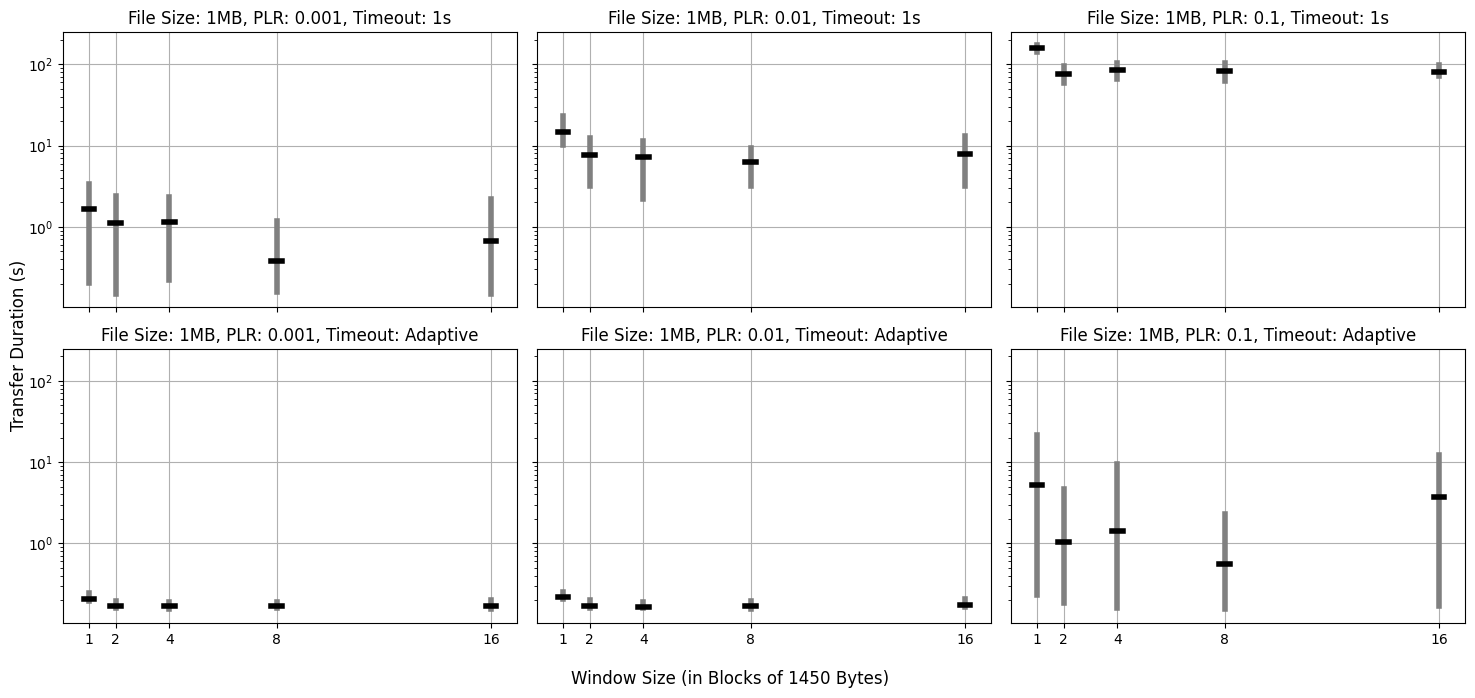
\includegraphics[width=1\textwidth]{benchmark1MB.png}
\end{figure}

\begin{figure}[H]
    \centering
    \begin{tabular}{|c|c|c|c|c|c|c|c|c|}
        \hline
        \rowcolor{tblhdrcolor}
        \multicolumn{1}{|c|}{\textbf{Dimensione File}}
                       & \multicolumn{1}{|c|}{\textbf{$T$}}
                       & \multicolumn{1}{|c|}{\textbf{$N$}}
                       & \multicolumn{1}{|c|}{\textbf{$p$}}
                       & \multicolumn{1}{|c|}{\textbf{Durata (min)}}
                       & \multicolumn{1}{|c|}{\textbf{Durata (avg)}}
                       & \multicolumn{1}{|c|}{\textbf{Durata (max)}}
        \\\hline
        10MB & 1s & 1 & 0.001 & 10.274 & 15.329 & 21.297\\\hline
        10MB & 1s & 2 & 0.001 & 7.677 & 10.437 & 16.011\\\hline
        10MB & 1s & 4 & 0.001 & 4.923 & 9.092 & 15.043\\\hline
        10MB & 1s & 8 & 0.001 & 3.888 & 8.690 & 12.273\\\hline
        10MB & 1s & 16 & 0.001 & 5.871 & 9.728 & 17.017\\\hline
        10MB & 1s & 1 & 0.01 & 137.437 & 149.161 & 158.904\\\hline
        10MB & 1s & 2 & 0.01 & 66.831 & 75.273 & 85.625\\\hline
        10MB & 1s & 4 & 0.01 & 65.319 & 76.243 & 83.083\\\hline
        10MB & 1s & 8 & 0.01 & 67.230 & 76.943 & 94.385\\\hline
        10MB & 1s & 16 & 0.01 & 63.062 & 86.293 & 155.677\\\hline
        10MB & 1s & 1 & 0.1 & 1558.596 & 1558.596 & 1558.596\\\hline
        10MB & 1s & 2 & 0.1 & 793.479 & 821.831 & 863.758\\\hline
        10MB & 1s & 4 & 0.1 & 827.607 & 827.607 & 827.607\\\hline
        10MB & 1s & 8 & 0.1 & 785.314 & 785.314 & 785.314\\\hline
        10MB & 1s & 16 & 0.1 & 802.164 & 802.164 & 802.164\\\hline
        10MB & $A$ & 1 & 0.001 & 1.963 & 2.038 & 2.263\\\hline
        10MB & $A$ & 2 & 0.001 & 1.587 & 1.611 & 1.639\\\hline
        10MB & $A$ & 4 & 0.001 & 1.548 & 1.584 & 1.619\\\hline
        10MB & $A$ & 8 & 0.001 & 1.576 & 1.602 & 1.624\\\hline
        10MB & $A$ & 16 & 0.001 & 1.596 & 1.684 & 1.949\\\hline
        10MB & $A$ & 1 & 0.01 & 2.031 & 2.139 & 2.250\\\hline
        10MB & $A$ & 2 & 0.01 & 1.807 & 1.867 & 1.988\\\hline
        10MB & $A$ & 4 & 0.01 & 1.764 & 1.865 & 2.059\\\hline
        10MB & $A$ & 8 & 0.01 & 1.782 & 1.899 & 2.092\\\hline
        10MB & $A$ & 16 & 0.01 & 1.719 & 1.913 & 2.818\\\hline
        10MB & $A$ & 1 & 0.1 & 2.691 & 4.341 & 11.706\\\hline
        10MB & $A$ & 2 & 0.1 & 1.981 & 3.415 & 15.418\\\hline
        10MB & $A$ & 4 & 0.1 & 1.774 & 5.376 & 33.431\\\hline
        10MB & $A$ & 8 & 0.1 & 2.476 & 9.603 & 27.438\\\hline
        10MB & $A$ & 16 & 0.1 & 22.161 & 41.741 & 76.662\\\hline
    \end{tabular}
    \vspace{1cm}
    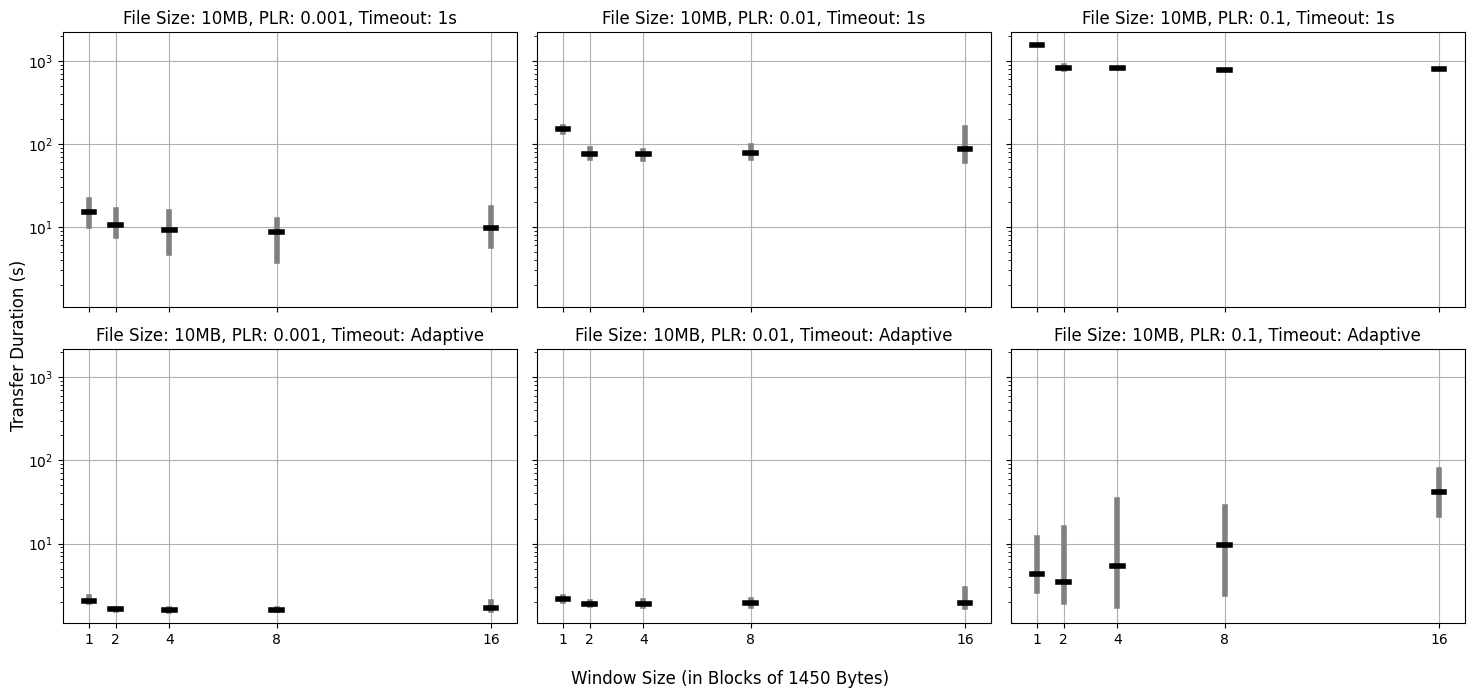
\includegraphics[width=1\textwidth]{benchmark10MB.png}
\end{figure}

\begin{figure}[H]
    \centering
    \begin{tabular}{|c|c|c|c|c|c|c|c|c|}
        \hline
        \rowcolor{tblhdrcolor}
        \multicolumn{1}{|c|}{\textbf{Dimensione File}}
                       & \multicolumn{1}{|c|}{\textbf{$T$}}
                       & \multicolumn{1}{|c|}{\textbf{$N$}}
                       & \multicolumn{1}{|c|}{\textbf{$p$}}
                       & \multicolumn{1}{|c|}{\textbf{Durata (min)}}
                       & \multicolumn{1}{|c|}{\textbf{Durata (avg)}}
                       & \multicolumn{1}{|c|}{\textbf{Durata (max)}}
        \\\hline
        100MB & 1s & 1 & 0.001 & 145.600 & 162.794 & 180.984\\\hline
        100MB & 1s & 2 & 0.001 & 71.801 & 87.836 & 105.588\\\hline
        100MB & 1s & 4 & 0.001 & 74.965 & 93.232 & 108.449\\\hline
        100MB & 1s & 8 & 0.001 & 79.147 & 90.768 & 105.707\\\hline
        100MB & 1s & 16 & 0.001 & 82.060 & 93.611 & 112.438\\\hline
        100MB & 1s & 1 & 0.01 & 1193.140 & 1193.140 & 1193.140\\\hline
        100MB & 1s & 2 & 0.01 & 424.000 & 424.000 & 424.000\\\hline
        100MB & 1s & 4 & 0.01 & 862.400 & 862.400 & 862.400\\\hline
        100MB & 1s & 8 & 0.01 & 987.700 & 987.700 & 987.700\\\hline
        100MB & 1s & 16 & 0.01 & 804.600 & 804.600 & 804.600\\\hline
        100MB & 1s & 1 & 0.1 & 15265.835 & 15265.835 & 15265.835\\\hline
        100MB & 1s & 2 & 0.1 & 8218.300 & 8218.300 & 8218.300\\\hline
        100MB & 1s & 4 & 0.1 & 8276.070 & 8276.070 & 8276.070\\\hline
        100MB & 1s & 8 & 0.1 & 7853.140 & 7853.140 & 7853.140\\\hline
        100MB & 1s & 16 & 0.1 & 7994.111 & 7994.111 & 7994.111\\\hline
        100MB & $A$ & 1 & 0.001 & 22.148 & 22.514 & 24.328\\\hline
        100MB & $A$ & 2 & 0.001 & 17.789 & 19.183 & 20.526\\\hline
        100MB & $A$ & 4 & 0.001 & 18.938 & 20.990 & 22.852\\\hline
        100MB & $A$ & 8 & 0.001 & 17.758 & 18.540 & 18.791\\\hline
        100MB & $A$ & 16 & 0.001 & 17.753 & 18.016 & 18.643\\\hline
        100MB & $A$ & 1 & 0.01 & 22.497 & 23.497 & 26.472\\\hline
        100MB & $A$ & 2 & 0.01 & 17.754 & 18.008 & 18.316\\\hline
        100MB & $A$ & 4 & 0.01 & 17.391 & 18.220 & 20.440\\\hline
        100MB & $A$ & 8 & 0.01 & 17.500 & 18.907 & 28.858\\\hline
        100MB & $A$ & 16 & 0.01 & 18.497 & 19.436 & 20.598\\\hline
        100MB & $A$ & 1 & 0.1 & 27.755 & 33.784 & 53.118\\\hline
        100MB & $A$ & 2 & 0.1 & 20.190 & 23.729 & 31.599\\\hline
        100MB & $A$ & 4 & 0.1 & 20.461 & 23.204 & 30.730\\\hline
        100MB & $A$ & 8 & 0.1 & 25.975 & 53.874 & 187.643\\\hline
        100MB & $A$ & 16 & 0.1 & 274.613 & 343.539 & 395.516\\\hline
    \end{tabular}
    \vspace{1cm}
    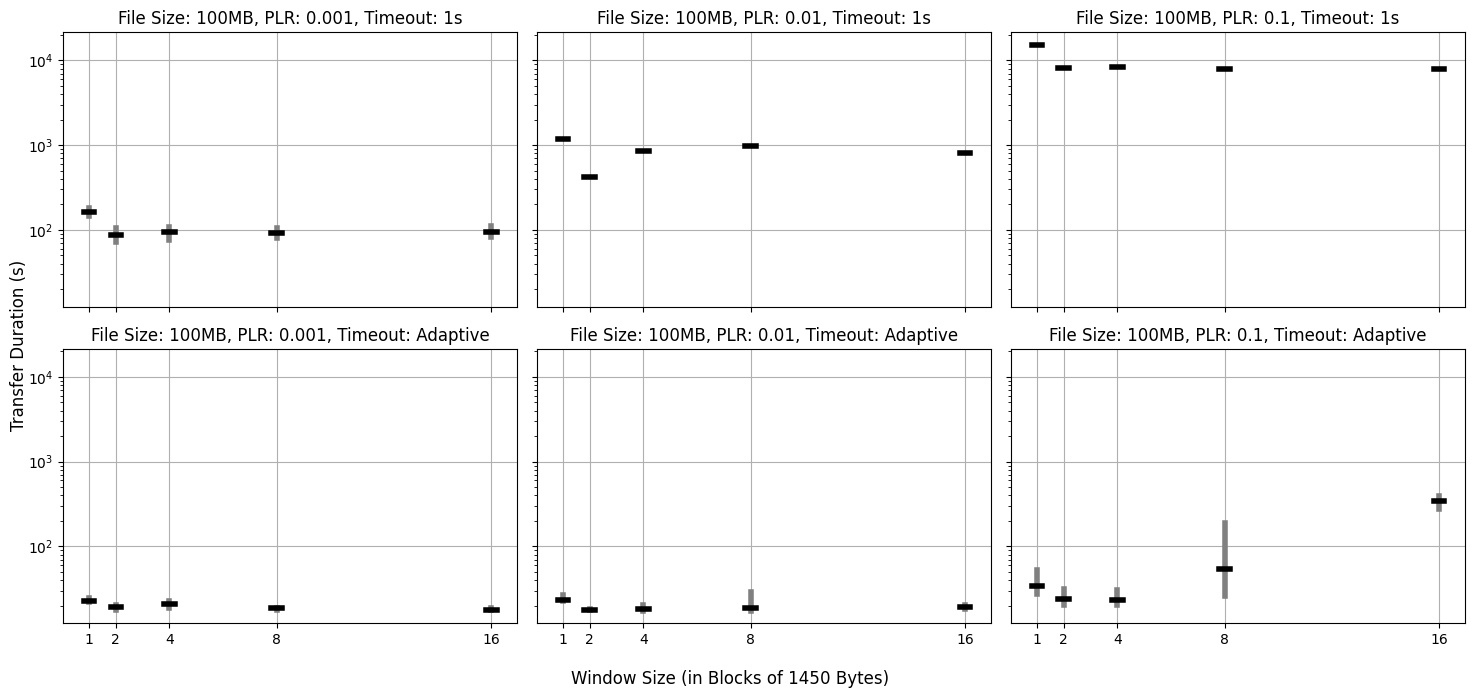
\includegraphics[width=1\textwidth]{benchmark100MB.png}
\end{figure}


Si osserva che, nel protocollo TFTP come definito nell'RFC 2349, essendo il valore minimo per il timeout pari a 1 secondo, l'impiego di un timeout adattivo può migliorare in modo significativo le prestazioni in reti soggette a elevati tassi di errore, come le reti wireless conformi allo standard IEEE 802.11 (Wi-Fi).

Notiamo inoltre come, variando le dimensioni della finestra di spedizione, non si riscontrano variazioni significative nella durata delle trasmissioni. Tale risultato è riconducibile alla modalità con cui sono stati condotti i test: utilizzando un unico nodo di rete sia come client sia come server, il ritardo di propagazione è stato completamente virtualizzato, consentendo il raggiungimento rapido della condizione di trasmissione continua. I risultati dei test effettuati non sono dunque rappresentativi delle prestazioni percepite su una rete ad alta latenza.

}

\section{Installazione, configurazione ed esecuzione} {

% manuale per l'installazione, la configurazione e l'esecuzione del sistema.

\subsection{Requisiti di Sistema}

Per garantire il corretto funzionamento del sistema, è necessario soddisfare i seguenti requisiti minimi:

\begin{itemize}
    \item \textbf{Sistema operativo:} distribuzione Linux compatibile.
    \item \textbf{Spazio su disco:} almeno 4 MB di spazio disponibile su disco.
    \item \textbf{Versione del kernel:} il server richiede un kernel Linux versione 6.1 o successiva per poter essere eseguito correttamente.
\end{itemize}

Il sistema di compilazione supporta ufficialmente la sola architettura \texttt{amd64}.
L'utilizzo di architetture diverse richiede azioni aggiuntive per la generazione di un preset valido per la compilazione.

\subsection{Procedura di Compilazione e Build}

Per poter compilare il progetto è necessario aver installato i seguenti programmi: \texttt{gdb}, \texttt{make}, \texttt{ninja-build}, \texttt{rsync}, \texttt{zip}, \texttt{cmake}, \texttt{g++} e \texttt{gcc} assicurandosi che la versione di gcc installata supporti C23.

Dopo aver scaricato i file sorgente del progetto clonando la relativa repository github, ed essersi spostati nella directory generata eseguendo da terminale i comandi
\begin{verbatim}
    git clone --recurse-submodules https://github.com/buracchi/tftp.git
    cd tftp
\end{verbatim}
è possibile compilare la soluzione eseguendo sempre da terminale i comandi
\begin{verbatim}
    cmake -S . --preset x64-linux-release
    cmake --build --preset x64-linux-release -j $(nproc)
\end{verbatim}
I file compilati saranno contenuti nella sottodirectory \texttt{build}. 

\pagebreak
\subsection{Installazione}

Nel caso in cui non si desideri compilare manualmente il software, è possibile scaricare semplicemente il tarball online contenente i binari precompilati eseguendo da terminale i comandi
\begin{verbatim}
    wget https://github.com/buracchi/tftp/releases/download/v1.0/tftp-1.0-x64.tar.gz
    tar -xzf tftp-1.0-x64.tar.gz
\end{verbatim}
Gli eseguibili saranno contenuti all'interno della directory \texttt{bin}.

\subsection{Manuale d'uso}

\subsubsection{TFTP Server}

Il TFTP Server espone numerose opzioni che consentono di configurare il comportamento operativo in base alle esigenze specifiche. Il comando di esecuzione di base è il seguente:
\begin{verbatim}
./server [OPTIONS] [directory]
\end{verbatim}
dove:
\begin{itemize}
    \item \texttt{directory ROOT:} Specifica la directory radice per lo storage dei file (default: directory corrente).
    \item \texttt{--enable-write-requests:} Abilita le richieste di scrittura.
    \item \texttt{--enable-list-requests:} Abilita le richieste di elenco file.
    \item \texttt{--enable-adaptive-timeout:} Abilita il timeout adattivo, basato sui ritardi di rete.
    \item \texttt{-w, --workers COUNT:} Imposta il numero di thread lavoratori (default: 7).
    \item \texttt{-m, --max-sessions-per-worker SESSIONS:} Definisce il numero massimo di sessioni per ciascun worker (default: 32).
\end{itemize}

Le impostazioni di rete possono essere personalizzate tramite:
\begin{itemize}
    \item \texttt{-H, --host ADDRESS:} Specifica l'indirizzo a cui il server si deve associare (default: ::).
    \item \texttt{-p, --port PORT:} Indica la porta su cui il server attende le connessioni (default: 6969).
    \item \texttt{-r, --retries RETRIES:} Definisce il numero di tentativi di ritrasmissione prima di interrompere la comunicazione (default: 5).
    \item \texttt{-t, --timeout SECONDS:} Imposta il timeout in secondi prima di una ritrasmissione (default: 2).
\end{itemize}

Per scopi di debug e simulazione, il server offre ulteriori opzioni:
\begin{itemize}
    \item \texttt{-l, --loss-probability PROBABILITY:} Configura la probabilità di simulare la perdita di pacchetti (default: 0.0).
    \item \texttt{--disable-fixed-seed:} Disabilita la scelta di un seme fisso per la generazione di numeri pseudocasuali durante la simulazione della perdita di pacchetti.
    \item \texttt{-v, --log-level LEVEL:} Specifica il livello di verbosità dei log (default: info).
\end{itemize}

\pagebreak
\subsubsection{TFTP Client}

Il TFTP Client, progettato per interagire con il server, supporta diverse modalità operative accessibili tramite specifici suottocomandi. Il comando base è:
\begin{verbatim}
./client [OPTIONS] host SUBCOMMAND
\end{verbatim}
dove \textbf{host} rappresenta l'indirizzo IP o il nome dell'host del server.

I sotto comandi supportati sono:
\setlist[itemize,2]{label=$\diamond$}
\begin{itemize}
    \item \texttt{get [OPTIONS] filename:} Scarica un file dal server. Le opzioni includono:
    \begin{itemize}
        \item \texttt{-m, --mode MODE:} Specifica la modalità di trasferimento (default: octet).
        \item \texttt{-o, --output OUTPUT\_FILE:} Imposta il nome del file di output.
    \end{itemize}
    \item \texttt{put [OPTIONS] filename:} Carica un file sul server. È disponibile l'opzione:
    \begin{itemize}
        \item \texttt{-m, --mode MODE:} Imposta la modalità di trasferimento (default: octet).
    \end{itemize}
    \item \texttt{list [OPTIONS] [directory]:} Richiede l'elenco dei file presenti in una directory sul server. Il parametro \texttt{directory} è opzionale (default: directory corrente) e può essere accompagnato dall'opzione:
    \begin{itemize}
        \item \texttt{-m, --mode MODE:} Specifica la modalità di trasferimento (default: octet).
    \end{itemize}
\end{itemize}

Altre opzioni comuni del client includono:
\begin{itemize}
    \item \texttt{-p, --port PORT:} Imposta la porta per la connessione (default: 6969).
    \item \texttt{-r, --retries RETRIES:} Definisce il numero di tentativi prima di interrompere l'operazione (default: 3).
    \item \texttt{-t, --timeout SECONDS:} Specifica il timeout in secondi per l'attesa di una risposta.
    \item \texttt{-b, --block-size BLOCK\_SIZE:} Imposta la dimensione del blocco dati per il trasferimento.
    \item \texttt{-w, --window-size WINDOW\_SIZE:} Configura la dimensione della finestra di dispatch.
    \item \texttt{-a, --adaptive-timeout:} Abilita il timeout adattivo, basato sui ritardi di rete.
    \item \texttt{--use-tsize:} Richiede la dimensione del file dal server.
    \item \texttt{-l, --loss-probability PROBABILITY:} Simula una determinata probabilità di perdita dei pacchetti (default: 0.0).
    \item \texttt{--disable-fixed-seed:} Disabilita la scelta di un seme fisso per la generazione di numeri pseudocasuali durante la simulazione della perdita di pacchetti.
    \item \texttt{-v, --log-level LEVEL:} Imposta il livello di dettaglio dei log (default: info).
\end{itemize}

}

\end{document}
